\documentclass[11pt,letterpaper]{article}

% Load some basic packages that are useful to have
% and that should be part of any LaTeX installation.
%
% be able to include figures
\usepackage{graphicx}
% get nice colors
\usepackage{xcolor}

% change default font to Palatino (looks nicer!)
\usepackage[latin1]{inputenc}
\usepackage{mathpazo}
\usepackage[T1]{fontenc}
% load some useful math symbols/fonts
\usepackage{latexsym,amsfonts,amsmath,amssymb}

% comfort package to easily set margins
\usepackage[top=1in, bottom=1in, left=1in, right=1in]{geometry}

\usepackage{courier}

% control some spacings
%
% spacing after a paragraph
\setlength{\parskip}{.15cm}
% indentation at the top of a new paragraph
\setlength{\parindent}{0.0cm}


\begin{document}

\begin{center}
\Large
Ay190 -- Final Project\\
Scott Barenfeld\\
Date: \today
\end{center}

\section{Introduction}
Radio interferometers allow information from multiple radio antennae to be 
combined, giving the interferometer as a whole much greater resolution than 
a single dish on its own.  Because radio telescopes measure the incoming 
electric field itself (as a voltage), instead of just its intensity, the 
amplitude and phase of the electric field is preserved.  In an array, the 
time-averaged product of the voltages measured by each pair of antennae is 
reported as a \emph{visibility}.  Between antennas $i$ and $j$, the 
visibility is defined as:

\begin{equation}\label{eq:vis}
\mathcal{V}=\int_{4\pi} \! A(\hat{r})I(\hat{r})e^{-2\pi i\nu\vec{B}\cdot\hat{r}/c} \, \mathrm{d}\Omega,
\end{equation} 

where $A$ is the beam pattern of an individual antenna (in this case, a Gaussian 
with $\sigma$=1 arcmin), $I$ is the intensity 
of the sky, $\nu$ is the frequency of the radiation, $\vec{B}$ is the baseline 
vector between $i$ and $j$ ($\vec{r_i}-\vec{r_j}$), and $\hat{r}$ is the 
direction along the line of sight.  In the limit of a narrow field of view, 
Equation \ref{eq:vis} can be rewritten using a change of variables as: 

\begin{equation}\label{eq:vis2}
\mathcal{V}(u,v)=\int_{-\infty}^{\infty} \! \int_{-\infty}^{\infty} \! \frac{A(l,m)I(l,m)}{\sqrt{1-l^2-m^2}}e^{-2\pi i(ul+vm)} \, \mathrm{d}l \, \mathrm{d}m,
\end{equation}
where $(u,v)$ is the baseline vector between the two antennae in units of 
wavelengths and $l$ and $m$ are the angles (in radians) on the sky relative 
to the line of sight.  Equation \ref{eq:vis2} is simply a two-dimensional 
Fourier transform.  Thus, an image of the intensity pattern on the sky can 
be generated from the inverse Fourier transform of the measured visibilities.

\begin{equation}\label{eq:vis3}
\mathcal{I}(l,m)=\int_{-\infty}^{\infty} \! \int_{-\infty}^{\infty} \! \frac{\sqrt{1-l^2-m^2}}{A(l,m)I(l,m)}e^{2\pi i(ul+vm)} \, \mathrm{d}u \, \mathrm{d}v,
\end{equation}  

\section{Setup}
For this project, Michael provided us with a list of antenna positions and a 
list of the amplitude and phase of the visibility for each antenna pair, such 
that the visibility is defined as:
\begin{equation}
\mathcal{V}=Ae^{i\phi}.
\end{equation}
After reading in these files, our first step was to turn the antenna positions 
into $(u,v)$ baseline vectors, which we did by dividing the difference in 
$x$ and $y$ positions for each antenna pair by the wavelength of the 
observations (1 cm).  We then combined the $(u,v)$ baselines for 
each pair of antennas with the corresponding visibilities into a 
single array, \texttt{uvvis}.

\section{Imaging with a DFT}

Using a Discrete Fourier Transform is relatively straight forward. The discretized version of ~\ref{eq:vis3} is simply
\begin{equation}\label{eq:vis3}
\mathcal{I}(l,m)= \Sigma_{u} \! \Sigma_{v} \! \frac{\sqrt{1-l^2-m^2}}{A(l,m)I(l,m)}e^{2\pi i(ul+vm)} \,
\end{equation}  

\section{Imaging with an FFT}
Python's built-in FFT and inverse-FFT functions expect the input 
to be on an evenly spaced grid.  So to form an image from the 
measured visibilities using an FFT, we first had to place the 
visibilities on such a grid.  We created a 100$\times$100 grid in 
the $(u,v)$ plane.  For each measured $u$ and $v$ value, we found the 
grid $u$ and $v$ it was closest to using Python's \texttt{bisect\_left} 
function.  This function returns the location of where a given value 
would be inserted in a sorted array.  So, given a measured $u$ or $v$, 
the closest grid $u$ or $v$ is one of the elements on either side of 
where the measured value would be inserted in the grid.  Subtracting the 
measured value from each of these two elements gives which grid element 
element is closest.  Once each measured $(u,v)$ is assigned to a 
gridpoint in this way, the visibility at each gridpoint is defined 
to be the sum of all the measured visibilities assigned to that gridpoint.

The gridded visibilities are then use to form an image.  From Equation 
\ref{eq:vis2}, it is easy to see that intensity is given by:
\begin{equation}
I(l,m)=\frac{\hat{\mathcal{V}}(l,m)\sqrt{1-l^2-m^2}}{A(l,m)},
\end{equation}
where $\hat{\mathcal{V}}(l,m)$ is the inverse-FFT of the gridded 
visibilities.  The resulting image is shown in Figure \ref{fig:fft}.

\begin{figure}[!h]
\centering
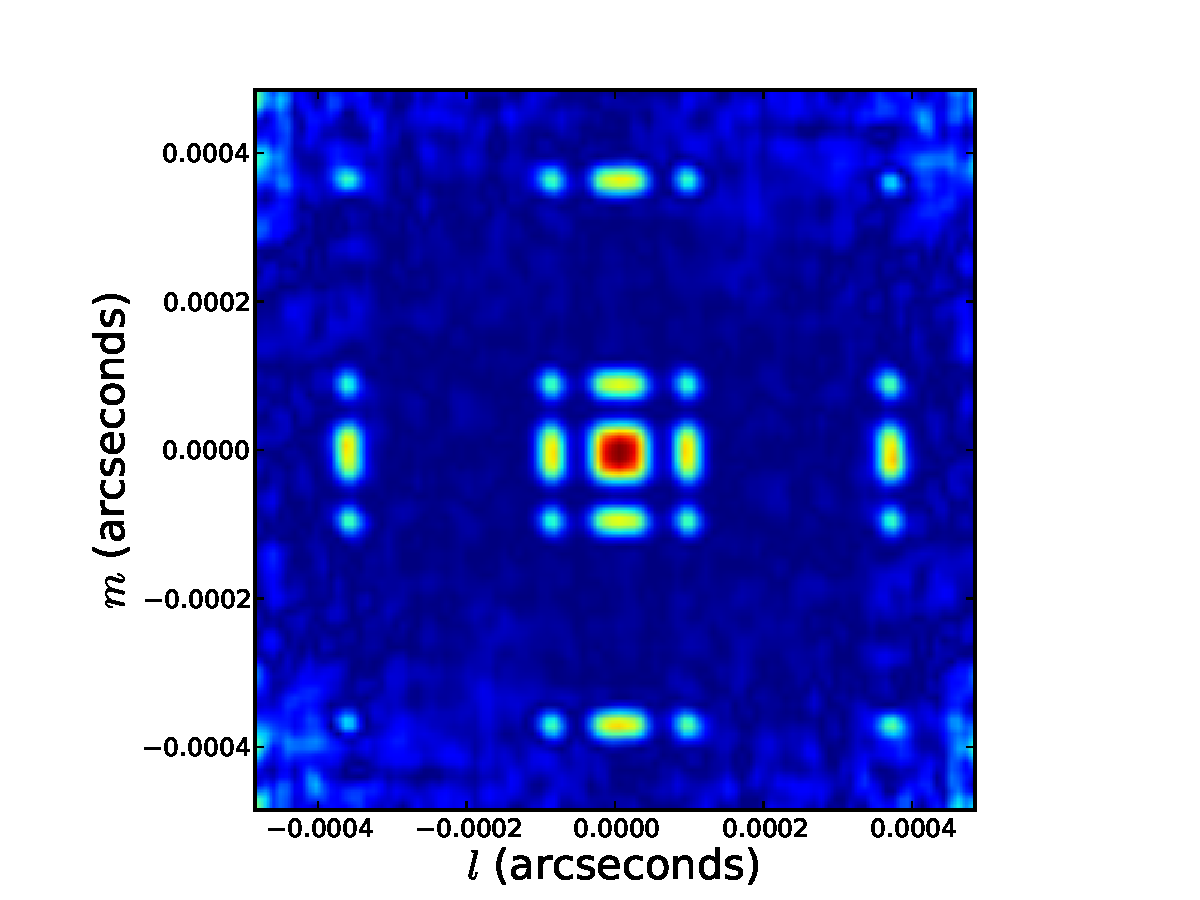
\includegraphics[width=0.5\textwidth]{FFT_Image.pdf}
\caption{Image created with an FFT using all 256 antennae.}
\label{fig:fft}
\end{figure}


\section{Discussion}


\end{document}

